\documentclass{article}
\usepackage{amsmath}
\usepackage{amssymb}
\usepackage{enumitem}
\usepackage{algorithm}
\usepackage{listings}
\usepackage{color,xcolor}
\usepackage[T1]{fontenc}
\usepackage{etoolbox}
\usepackage{multicol}
\usepackage{geometry}
\usepackage[colorlinks=true,linkcolor=blue,urlcolor=red,bookmarksopen=true]{hyperref}
\usepackage{tikz, pgfplots, tkz-euclide,calc}
    \usetikzlibrary{patterns,snakes,shapes.arrows,3d}
    \geometry{
        total = {160mm, 237mm},
        left = 25mm,
        right = 35mm,
        top = 30mm,
        bottom = 30mm,
      }

\usepackage{tcolorbox}
     \tcbuselibrary{listings,skins}

\newcommand{\enter}{\raisebox{-1.8pt}{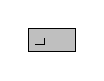
\begin{tikzpicture}[scale=0.3]
    \draw[thin,fill=lightgray] (0,0) rectangle (2,1);
    \draw (0.3,0.3) -- (0.7,0.3)--(0.7,0.6);     
\end{tikzpicture}}}

\definecolor{pgray}{rgb}{0.5,0.5,0.5}
\definecolor{pblue}{rgb}{0.13,0.13,1}
\definecolor{pgreen}{rgb}{0,0.5,0}
\definecolor{pred}{rgb}{0.9,0,0}
\definecolor{pgrey}{rgb}{0.46,0.45,0.48}
\definecolor{pcyan}{HTML}{D4EFFC}
\definecolor{lblue}{HTML}{00AEEF}
\definecolor{input}{HTML}{AAE1FA}
\definecolor{bg}{rgb}{0.95, 0.95, 0.92}
\definecolor{vscode}{HTML}{282A36}
\definecolor{PastelGreen}{HTML}{77DD77}

\newcommand{\nextline}[1]{\raisebox{0pt}[1pt]{\colorbox{input}{#1}}}

\usepackage{listings}

\lstdefinestyle{Liang}{
language=Java,
showspaces=false,
showtabs=false,
breaklines=true,
showstringspaces=false,
breakatwhitespace=true,
commentstyle=\color{pgray},
keywordstyle=\color{pblue},
stringstyle=\color{pgreen},
basicstyle=\small\ttfamily,
frame=single,
backgroundcolor=\color{pcyan},
escapeinside={(*}{*)},}

\lstdefinestyle{output}{
    language=Java,
    backgroundcolor=\color{vscode},
    basicstyle=\small\ttfamily\color{white},
    frame=none,
    escapeinside={(*}{*)},
    showspaces=false,
    showtabs=false,
    breaklines=true,
    showstringspaces=false,
    breakatwhitespace=true,
    keywordstyle=\color{white},
    }

\lstdefinestyle{standard}{
    language=Java,
    showspaces=false,
    showtabs=false,
    breaklines=true,
    showstringspaces=false,
    breakatwhitespace=true,
    commentstyle=\color{pgray},
    keywordstyle=\color{pblue},
    stringstyle=\color{pgreen},
    basicstyle=\small\ttfamily,
    frame=single,
    backgroundcolor=\color{bg},
    escapeinside={(*}{*)},}
\lstset{style=Liang}

\newtcblisting{RunCode}[2][enhanced,drop shadow]{
    arc=0pt, outer arc=0pt,
    boxsep=1pt,
    boxrule=2pt,
    auto outer arc,
    colback=vscode,
    colframe=bg,
    listing only, 
    listing style=output,
    title=\color{black}Ex. Output,
    #1
    }

    \newtcolorbox{hint}[2][]{
        colback=PastelGreen!5!white, 
        colframe=PastelGreen!75!black,
        fonttitle=\bfseries, 
        colbacktitle=PastelGreen!85!black,
        enhanced, 
        attach boxed title to top left={yshift=-2mm}, 
        title=Hint,
        #1
    }

\renewcommand{\thesubsection}{\arabic{subsection}}

\title{\textbf{Week 2 Assigment}}
\date{20 September 2024}
\author{Teosofi H.A \& Hafidz M.}

\begin{document}
    \maketitle
    \pagenumbering{gobble}

    \section*{Tugas Mandiri}
    \begin{enumerate}[label=\textbf{\arabic*.}]
        \item \textbf{(Geometri Analitik)}\\
        Diketahui sebuah persamaan lingkaran berpusat di titik $(h,k)$ dan berjari-jari $r$. Buatlah program untuk menampilkan persamaan lingkaran dengan bentuk
        \[x^2+y^2+Ax+By+C=0\]
        \begin{RunCode}{}
Titik pusat lingkaran di (2,3) dan berjari-jari 5.
Persamaan lingkarannya adalah x^2 + y^2 - 4x - 6y -12 = 0
        \end{RunCode}
        \begin{hint}[]{}
            Gunakan persamaan lingkaran umum $x^2+y^2+Ax+By+C=0$ dan substitusi $A=-2h$, $B=-2k$, dan $C=h^2+k^2-r^2$.
        \end{hint}
          
        \item \textbf{(Logika Matematika)}\\
        Kita tahu bahwa variabel $p$ dan $q$ yang dapat bernilai "benar" atau "salah" mempunyai 4 kemungkinan pasangan berbeda (BB, BS, SB, dan SS). Buatlah program untuk membuat tabel kebenaran dari salah satu ekspresi logika berikut\footnote{Cukup kerjakan satu abjad saja sesuai dengan kelas Alpro 1 anda}
        \begin{enumerate}[label=$\boxed{\text{\Alph*}}$]
            \item $\neg(p \land q) \Leftrightarrow \neg p \lor \neg q$  
            \item $\neg(p \lor q) \Leftrightarrow \neg p \land \neg q$ 
            \item $(p \lor q)\land \neg p \Leftrightarrow q$
            \item $(p \lor q)\land \neg q \Leftrightarrow p$
        \end{enumerate}
        Contoh: Tabel kebenaran $p\Leftrightarrow \neg\, p \land q$
        \begin{table}[h!]
            \centering
            \begin{tabular}{|c|c|c|c|c|}
                \hline
                $p$ & $q$ & $\neg\, p$ & $\neg\, p \land q$ & $p \Leftrightarrow \neg\, p \land q$\\
                \hline
                B & B & S & S & S\\
                B & S & S & S & S\\
                S & B & B & B & S\\
                S & S & B & S & B\\
                \hline
            \end{tabular}
        \end{table}
        \begin{RunCode}{}
|   p   |   q   |  !p   | !p ^ q | p <=> (!p ^ q) |
|-------|-------|-------|--------|----------------|
| true  | true  | false | false  | false          |
| true  | false | false | false  | false          |
| false | true  | true  | true   | false          |
| false | false | true  | false  | true           |
        \end{RunCode}

        \item \textbf{(Metode Statistika)}\\
        Diberikan variabel acak $X$ yang mempunyai distribusi peluang sebagai berikut.
        \begin{center}
            \begin{tabular}{|c|c|c|c|c|c|}
                \hline
                $x$ & 2 & 3 & 6 & 7 & 9\\
                \hline
                $P(X=x)$ & 0.1 & 0.2 & 0.3 & 0.2 & 0.2\\
                \hline
            \end{tabular}
        \end{center}
        Buatlah program untuk menampilan ekspektasi dan varians dari variabel acak $X$.
        \begin{RunCode}{}
Ekspektasi dari variabel acak X adalah 5.8
Varians dari variabel acak X adalah 5.359999999999999
        \end{RunCode}
        \begin{hint}[]{}
            Buatlah variabel untuk $x_1, x_2, \ldots, x_n$ dan $p_1, p_2, \ldots, p_n$ (nilainya harus saling bersesuaian). Kemudian hitung ekspektasi dan varians dengan rumus
            \begin{itemize}
                \item Ekspektasi: $\mu = E(X) = \sum_{i=1}^{n} x_i \cdot p_i$
                \item Varians: $\sigma^2 = Var(X) = \sum_{i=1}^{n} (x_i - \mu)^2 \cdot p_i$
            \end{itemize}
        \end{hint}
    \end{enumerate}
\end{document}